\clanguage

\chapter{Utilisation de la bibliothèque sur une section critique}

Ici, l'enjeu est de constater que lorsque deux processus distincts utilisent une même zone de mémoire partagée (lecture puis écriture), on ne peut assurer l'intégrité des données sans sémaphore. En effet, nous allons constater qu'entre le moment où un processus lit une donnée partagée et le moment où il l'écrase, celle-ci a pu changer entre temps (modifiée par un autre processus).

\section{Zone critique sans sémaphore}

\subsection{\lstinline{main()}}

Voici le code de la fonction \lstinline{main()} qui fait le \lstinline{fork()} et lance la boucle de 100 itérations (fonction \lstinline{afaire(int isFather))} pour les deux processus.

\textcode{excl-mutu-none.c}
\begin{lstlisting}
...
int main() {
    shmid = shmget(IPC_PRIVATE,sizeof(int),IPC_CREAT|IPC_EXCL|0666); // Création d'un espace de mémoire partagé de la taille de 1 int
    adr = (int*) shmat(shmid,NULL,0); // Shell memory attachment
    *adr = 0;
    srand(time(NULL));
    switch (son = fork()) {
        case 0:
            printf("%d Fils créé\n",getpid());
            afaire(0);
            shmdt(adr); // détache le segment
            break;
        case -1:
            printf("Erreur\n");
            exit(0);
        default:
            printf("%d Père créé.\n",getpid());
            afaire(1);
            wait();
            printf("Valeur finale affichée par le père après fin du fils:\t%d\n",*adr);
            shmdt(adr); // détache le segment
            shmctl(shmid,IPC_RMID,0); // Shell memory control : permet de supprimer la mémoire partagée
    }
    return 0;
}
\end{lstlisting}

\subsection{\lstinline{afaire(int isFather)}}

Et voici la fonction \lstinline{afaire(int isFather)} qui fait les 100 itérations. Pour chaque itération, voici ce qui est fait :
\begin{enumerate}
  \item Affecter E à une variable A, entière, locale au process.
  \item Attendre entre 20 et 100 ms
  \item Incrémenter A.
  \item Affecter la variable locale A à la variable "partagée" E.
  \item Attendre entre 20 et 100 ms
  \item Affichage dans le process père de la valeur de E.
\end{enumerate}

\medskip

L'argument \lstinline{int isFather} de la fonction \lstinline{void afaire(int isFather)} permet de savoir si le processus qui appelle cette fonction est le processus père ou non. Si tel est le cas, alors celui-ci affiche à chaque fin d'itération la valeur de E (entier partagé).

\begin{lstlisting}
void afaire(int isFather) {
    int j;
    for (j = 0; j<100;j++) {
        var_locale = *adr; // récupération de l'entier partagé
        usleep((rand()%81) + 20); // temps d'attente entre 20 et 100ms
        var_locale++;
        *adr = var_locale; // normalement, *adr vaut *adr + 1, mais ce n'est pas sûr...
        usleep((rand()%81) + 20); // temps d'attente entre 20 et 100ms
        if (isFather == 1) printf("It %d:\t%d\n",j,*adr);
    }
}
\end{lstlisting}

\subsection{Sortie du programme sans sémaphore}

\begin{figure}[h!]
  \centering
  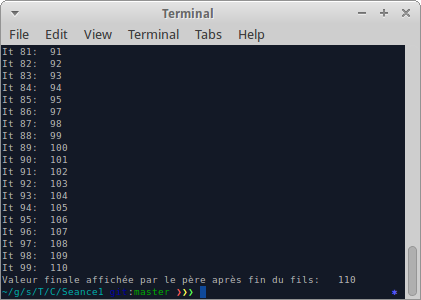
\includegraphics[width=0.66\textwidth]{seance2_img1.png}
  \caption{Sortie du programme}
\end{figure}

On constate qu'à chaque itération du père, la valeur lue sur le segment partagée ne correspond pas au numéro de l'itération. Cela s'explique par le fait que l'exécution du père peut être interrompue par le CPU pour laisser le fils s'exécuter. Or le fils incrémente lui aussi cet entier partagé. Lorsque le fils et le père ont fini des s'exécuter, après les deux itérations de 100 tours donc, le père affiche la valeur de l'entier partagé. \textbf{On constate ici le problème : l'entier devrait valoir 200 (100*2 incrémentations) or ce n'est jamais le cas.}

\section{Ajout d'un sémaphore}

La solution à ce problème est d'ajouter un sémaphore d'exclusion mutuelle (qui vaut 1). Avant chaque accès à la zone critique (lecture) et jusqu'à l'écriture du nouvel entier partagé, on décremente le sémaphore (cela bloque donc les autres processus qui faire la même chose). Après l'écriture du nouvel entier partagé, on l'incrémente à nouveau de 1. Ainsi les autres processus peuvent à leur tour décrémenter le sémaphore et modifier l'entier partagé, et ainsi de suite.

\subsection{Code corrigé}

\textcode{excl-mutu.c}
\begin{lstlisting}
...
void afaire(int isFather) {
    int j;
    for (j = 0; j<100;j++) {
        P(0); // Début de zone critique
        // Incrémentation de l'entier partagé grâce à la variable locale
        V(0); // Fin de zone critique
        usleep((rand()%81) + 20);
        if (isFather == 1) printf("It %d:\t%d\n",j,*adr);
    }
}

int main() {
    ...
    init_semaphore();
    val_sem(0,1);
    switch (son = fork()) {
        case 0:
            ...
        case -1:
            ...
        default:
            ...
            detruire_semaphore();
    }
    return 0;
}
\end{lstlisting}

\subsection{Sortie du programme avec sémaphore}

On constate dans le screenshot ci-desous que la valeur finale de l'entier partagé est 200, ce qui est la valeur attendue. À chaque fois que le fils ou le père ont lu et modifié l'entier partagé, ils se sont exclus mutullement (bloqués). Ainsi, aucun processus ne pouvait modifier l'entier partagé alors que l'autre n'avait pas fini de le modifier.

\begin{figure}[h!]
  \centering
  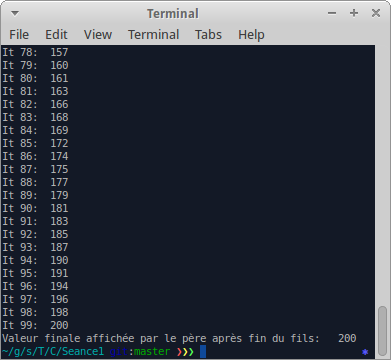
\includegraphics[width=0.66\textwidth]{seance2_img2.png}
  \caption{Sortie du programme}
\end{figure}

\chapter{Utilisation de la bibliothèque pour un producteur-consommateur}

Le but de cet exercice est de produire et consommer (par deux processus respectivement différents) des entiers contenus un tableau (en mémoire partagée) circulaire de taille 5. Le producteur doit s'arrêter quand le tableau est plein (et attendre qu'il y ait une place libre avant de le remplir à nouveau) et inversement pour le consommateur, il ne doit \og consommer\fg{} que s'il y a au moins une place occupée (donc si le tableau n'est pas vide). \textbf{Cela se met en \oe{}uvre grâce à deux sémaphores :}
\begin{itemize}
  \item Un sémaphore correspondra aux emplacements libres dans le tableau, il sera donc initialisé à 5 et sera décrémenté à chaque fois qu'un entier est produit
  \item Un sémaphore correspondra aux emplacement occupés dans le tableau, il sera donc initialisé à 0 et sera incrémenté à chaque fois qu'un entier est produit
\end{itemize}

\section{Rôles du consommateur et du producteur}
Par conséquent, le consommateur incrémentera le sémaphore des places libres et décrémentera celui des places occupées à chaque fois qu'il lira un entier. Le producteur fera l'inverse à chaque fois qu'il écrira un nouvel entier.

\medskip

Quand il n'y aura plus de place libre, le producteur se verra bloqué lorsqu'il essaiera de décrementer le sémaphore. De même, lorsqu'il n'y aura plus de place occupée, le consommmateur sera verra bloqué lorsqu'il essaiera de décrémenter le sémaphore. \textbf{Les contraintes du sujet de l'excercice sont donc respectées.}

\section{Index de lecture et d'écriture}

Un index \lstinline{int i} propre au consommateur et au producteur sera incrémenté à chaque fois que l'un ou l'autre produira ou consommera. De manière à avoir un tableau circulaire, cet index sera toujours \og lu\fg{} modulo 5.

\section{Code}

\textcode{prod-conso.c}
\begin{lstlisting}
#include <stdio.h>
#include <stdlib.h>
#include <sys/types.h>
#include <sys/ipc.h>
#include <sys/shm.h>
#include <unistd.h>

// CONSTANTES (noms des sémaphores)
int const SEM_PLACES_LIBRES = 0;
int const SEM_PLACES_OCCUPEES = 1;

int shmid;
int *adr;

int main() {
    int i;
    shmid = shmget(IPC_PRIVATE,5*sizeof(int),IPC_CREAT|IPC_EXCL|0666); // Création d'un espace de mémoire partagé de taille 5 entiers
    adr = (int*) shmat(shmid,NULL,0); // Shell memory attachment

    // Initialisations des 2 sémaphores avec leurs valeurs
    init_semaphore();
    val_sem(SEM_PLACES_LIBRES,5);
    val_sem(SEM_PLACES_OCCUPEES,0);

    srand(time(NULL));

    switch (fork()) {
        case 0:
            printf("%d Fils créé\n",getpid()); // producteur
            int tmp;
            for (i = 0; i<10; i++) { // On aurait pu faire un while(true)
                P(SEM_PLACES_LIBRES);
                tmp = (rand()%50) + 1;
                adr[i%5] = tmp;
                printf("Ajouté: %d\n",tmp);
                V(SEM_PLACES_OCCUPEES);
            }
            shmdt(adr); // détache le segment
            break;
        case -1:
            printf("Erreur\n");
            exit(0);
        default:
            printf("%d Père créé.\n",getpid()); // consommateur
            for (i = 0; i<10; i++) { // On aurait pu faire un while(true)
                P(SEM_PLACES_OCCUPEES);
                printf("Consommé: %d\n",adr[i%5]);
                V(SEM_PLACES_LIBRES);
            }
            shmdt(adr); // détache le segment
            shmctl(shmid,IPC_RMID,0); // Shell memory control : permet de supprimer la mémoire partagée
            detruire_semaphore();
    }
    return 0;
}
\end{lstlisting}

\section{Sortie du programme}

Voici la sortie du programme (ci-dessous). On constate que le fils produit les 5 entiers jusqu'à ce que le tableau soit plein, avant que le CPU ne laisse le père s'exécuter. On constate que l'ordre de création (production) des entiers correspond bien à l'ordre de lecture (consommation), les index fonctionnent donc bien. Enfin, chaque processus s'arrête si le tableau est vide ou plein : la contrainte est respectée.

\begin{figure}[h!]
  \centering
  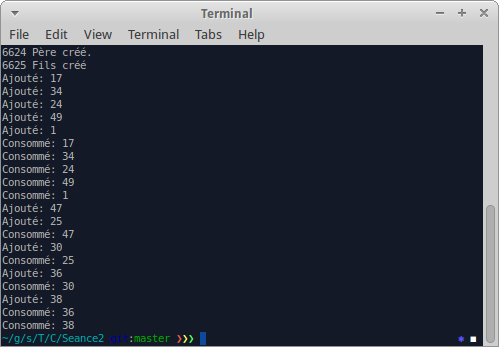
\includegraphics[width=0.66\textwidth]{seance2_img3.png}
  \caption{Sortie du programme}
\end{figure}